%% LaTeX2e class for student theses
%% thesis.tex
%% 
%% Karlsruhe Institute of Technology
%% Institute for Program Structures and Data Organization
%% Chair for Software Design and Quality (SDQ)
%%
%% Dr.-Ing. Erik Burger
%% burger@kit.edu
%%
%% See https://sdqweb.ipd.kit.edu/wiki/Dokumentvorlagen
%%
%% Version 1.3.5, 2020-06-26

%% Available page modes: oneside, twoside
%% Available languages: english, ngerman
%% Available modes: draft, final (see README)
\documentclass[oneside, english]{sdqthesis}

%% ---------------------------------
%% | Information about the thesis  |
%% ---------------------------------

%% Name of the author
\author{Christoph Stelz}

%% Title (and possibly subtitle) of the thesis
\title{Core-Count Independent Reproducible Reduce}

%% Type of the thesis 
\thesistype{Bachelor's Thesis}

%% Change the institute here, ``IPD'' is default
\myinstitute{Institute of Theoretical Informatics}

%% You can put a logo in the ``logos'' directory and include it here
%% instead of the SDQ logo
% \grouplogo{myfile}
%% Alternatively, you can disable the group logo
\nogrouplogo

%% The reviewers are the professors that grade your thesis
\reviewerone{Prof. Dr. Alexandros Stamatakis}
\reviewertwo{Prof. Dr. Peter Sanders}

%% The advisors are PhDs or Postdocs
\advisorone{M.Sc. Lukas Hübner}
%% The second advisor can be omitted
%\advisortwo{M.Sc. D}

%% Please enter the start end end time of your thesis
\editingtime{01. December 2021}{01. April 2022}

\settitle

%% --------------------------------
%% | Settings for word separation |
%% --------------------------------

%% Describe separation hints here.
%% For more details, see 
%% http://en.wikibooks.org/wiki/LaTeX/Text_Formatting#Hyphenation
\hyphenation{
% me-ta-mo-del
}

%% --------------------------------
%% | Bibliography                 |
%% --------------------------------

%% Use biber instead of BibTeX, see README
\usepackage[citestyle=numeric,style=numeric,backend=biber]{biblatex}
\usepackage{tikz}
\usepackage{pgffor}
\usetikzlibrary {graphs}
\usepackage{luacode}


\directlua{dofile("scripts/tree.lua")}

\newcommand{\F}{\mathbb{F}}

\addbibresource{thesis.bib}

%% ====================================
%% ====================================
%% ||                                ||
%% || Beginning of the main document ||
%% ||                                ||
%% ====================================
%% ====================================
\begin{document}

%% Set PDF metadata
\setpdf

%% Set the title
\maketitle

%% The Preamble begins here
\frontmatter

%% LaTeX2e class for student theses: Declaration of independent work
%% sections/declaration.tex
%% 
%% Karlsruhe Institute of Technology
%% Institute for Program Structures and Data Organization
%% Chair for Software Design and Quality (SDQ)
%%
%% Dr.-Ing. Erik Burger
%% burger@kit.edu
%%
%% Version 1.3.5, 2020-06-26

\thispagestyle{empty}
\null\vfill
\noindent\hbox to \textwidth{\hrulefill} 
\iflanguage{english}{I declare that I have developed and written the enclosed
thesis completely by myself, and have not used sources or means without
declaration in the text.}%
{Ich versichere wahrheitsgemäß, die Arbeit
selbstständig angefertigt, alle benutzten Hilfsmittel vollständig und genau
angegeben und alles kenntlich gemacht zu haben, was aus Arbeiten anderer
unverändert oder mit Änderungen entnommen wurde.}
 
 
%% ---------------------------------------------
%% | Replace PLACE and DATE with actual values |
%% ---------------------------------------------
\textbf{Karlsruhe, 01.04.2022}
\vspace{1.5cm}
 
\dotfill\hspace*{8.0cm}\\
\hspace*{2cm}(\theauthor) 
\cleardoublepage


\setcounter{page}{1}
\pagenumbering{roman}

%% ----------------
%% |   Abstract   |
%% ----------------
 
%% For theses written in English, an abstract both in English
%% and German is mandatory.
%%
%% For theses written in German, a German abstract is sufficient.
%%
%% The text is included from the following files:
%% - sections/abstract

\includeabstract

%% ------------------------
%% |   Table of Contents  |
%% ------------------------
\tableofcontents

\listoffigures
\listoftables

%% -----------------
%% |   Main part   |
%% -----------------

\mainmatter

\chapter{Introduction}
\label{ch:Introduction}

\section{Motivation}
\label{sec:Motivation}
A common problem in massively parallel computations is the reduction (for example summation) of results over the entire cluster.
Widespread implementations do not account for cluster-size-independent reproducibility and will deliver different results
even if the only variable element is the number of participating \glsfirstplural{pe}.

RAxML-NG~\cite{kozlov_raxml-ng_2019-1} for example is a software package that estimates phylogenetic trees based on a multiple sequence alignment (MSA) from different taxa.
Given the exponentially large number of possible trees (for $100$ taxa there exist over $10^{182}$ distinct phylogenies~\cite{stamatakis_efficient_2020}) and proven $\mathcal{NP}$-hardness of the problem~\cite{roch_short_2006}, a complete tree search is infeasible.
Instead, RAxML-NG uses stochastic evolutionary models to determine the likelihood of a given tree and performs a tree search to find a maximum likelihood estimate.
Because of their small magnitude, programs usually deal with likelihood values logarithmically.
To increase execution speed, RAxML-NG assumes that different sites evolve independently and computes per-site likelihoods in parallel on different threads.
The overall likelihood of a tree is the product of all per-site likelihoods, therefore the tree log-likelihood is the sum of all per-site log-likelihoods (PSLLHs):
\begin{align}
L_{\textrm{tree}} &= \prod_{s \in \textrm{sites}} L_s \\
\label{eq:llh_sum}
\log L_{\textrm{tree}} &= \log (\prod_{s \in \textrm{sites}} L_s) = \sum_{s \in \textrm{sites}}  \log L_s
\end{align}
During the tree search, the log-likelihoods determine the alteration of a tree in order to further increase its likelihood.
Therefore, the correctness of sum \eqref{eq:llh_sum} is critically important for the resulting trees.
RAxML-NG uses floating-point numbers to represent LLH values, but floating-point arithmetic is not necessarily associative due to rounding errors~\cite{goldberg_what_1991}.
Darriba et al.\ have shown that executing the same version of RAxML-NG with the same input data and same random seed can still produce different trees by varying the number of threads, because of the different summation orders~\cite{darriba_state_2018}.

\section{Preliminaries}
\label{sec:Preliminaries}
Let $\F$ be the set of floating-point numbers. Given
\begin{itemize}
\item a cluster of $p$ \glspl{pe} indexed with a rank $i \in \{0, \ldots, p - 1\}$ and interconnected by a \gls{mpi}
\item $n_i$ floating-point numbers (elements) on the \gls{pe} with index $i$ ($N := \sum_{i=0}^{p-1} n_i$ in total)
\item a not necessarily associative binary operation $\circ: \F \times \F \rightarrow \F$
\end{itemize}
we want to reduce all numbers by means of $\circ$ so that the end result is bitwise-reproducible.
A reduction algorithm is bitwise-reproducible if multiple executions over the same set of numbers with a variable number of \glspl{pe} produce bit-per-bit identical results.

In order to correctly distribute the $N$ elements over $p$ \glspl{pe}, we need to deal with cases where $N$ is not divisible by $p$.
Let $a := \lfloor \tfrac{N}{p} \rfloor$ be the rounded number of elements per \gls{pe}.
We can assign the remaining $N \bmod p$ elements to the upper or lower processes:
\begin{align}
\label{eq:lowerDistribution}
n_i^{\textrm{lower}} &= \begin{cases}
    a + 1 & \textrm{if } i < N \bmod p \\
    a & \textrm{otherwise}
\end{cases} \\
\label{eq:upperDistribution}
n_i^{\textrm{upper}} &= \begin{cases}
    a & \textrm{if } i < N - (N \bmod p) \\
    a + 1 & \textrm{otherwise}
\end{cases}
\end{align}

\section{Related Work}
\label{sec:RelatedWork}
Because of the abundance of reduction operations in modern high-performance-computing applications, there already exist multiple reproducible reduction algorithms.


\subsection{Sequential left-to-right reduction}
\label{sec:SequentialLeftToRightReduction}

A naive approach to solving above problem is to gather all elements on a single PE and then apply the reduction operation strictly from left to right:

\begin{equation}
x_0 \circ x_1 \circ x_2 \circ \ldots  \circ x_{N-1} = ((x_0 \circ x_1) \circ x_2) \circ \ldots
\end{equation}

While simple in implementation, this approach does not benefit from parallelization.
Because of the communication overhead, performance decreases with an increasing number of \glspl{pe}.


\subsection{Reproducible Accumulators}
\label{sec:Reproducible Accumulators}
For floating-point summation in particular, Ahrens et al.~\cite{ahrens_algorithms_2020} have developed an algorithm that uses a 48 Byte reproducible accumulator to avoid unpredictable rounding errors.
After reading all the input data, the summation can occur in parallel in no particular order and still produces bitwise identical results.
This requires around $9N$ floating-point operations and $3N$ bitwise operations.
The Reproducible Basic Linear Algebra Subprograms (ReproBLAS) software package implements this algorithm and exposes it via a user-friendly API.\@

This approach is not suitable for general reduction operations, since it depends on specific properties of floating-point numbers as specified in the IEEE 754 standard~\cite{noauthor_ieee_nodate} and is specific to summation.


\subsection{Reduction Tree}
\label{sec:ReductionTree}

\begin{figure}[H]
\centering
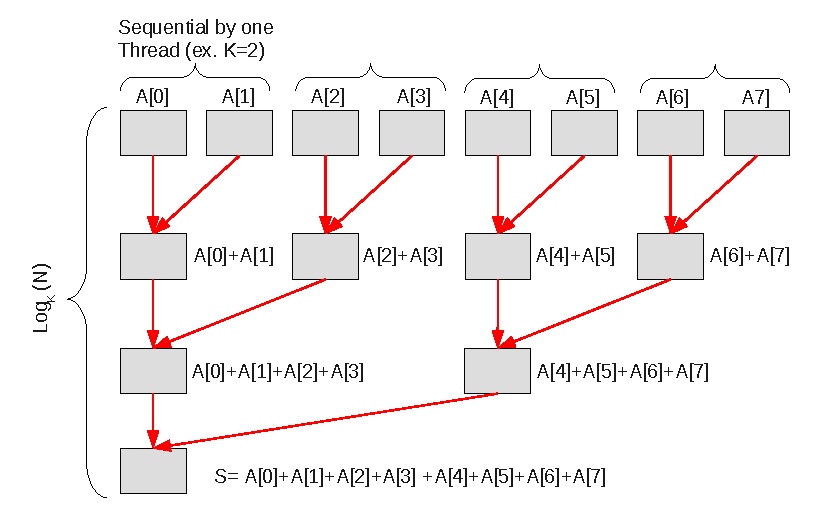
\includegraphics[scale=0.7]{figures/villa_et_al_reduction_tree.pdf}
\caption{General reduction tree (figure from Villa et al.\ \cite{villa_effects_2009}).}
\label{fig:villa_reduction_tree}
\end{figure}


Villa et al.~\cite{villa_effects_2009} utilize a $K$-ary tree structure on a Cray XMT system to sum floating-point numbers reproducibly (\Cref{fig:villa_reduction_tree}).
Using parallel-prefix accumulation, they compute the sum of $N$ summands in $\log_K (N)$ steps, where $K$ determines the amount of numbers the algorithm accumulates sequentially in each step.
The reproducibility stems from the fact that the reduction tree depends only on the total number of summands $N$ and the constant $K$, therefore the algorithm uses the same calculation order if the core-count differs.

The original source code is not available even after contacting the authors, therefore the implementation details are unknown and runtime comparisons impossible.

\chapter{Implementation}
\label{ch:Implementation}

In this chapter, we deduce the necessary equations to implement the reduction algorithm and present multiple optimizations.
We focus on summation, the reduction operator $\reduce$ will be floating-point addition.
While the recursive formula given in \Cref{eq:nodeReduceReduction} already defines a reduction algorithm, its implementation in imperative languages would heavily rely on the call stack to store intermediate results.
In practice, reducing iteratively from leaf nodes to the root yields faster runtimes.\footnote{For $N=2^{27}$ elements on $p=1$ \gls{pe}, we observe a $4.9$ speedup of the recursive reduction (Microbenchmark ID 5).}

The binary representation of element indices has $\numLevels$ bits.
If we order them from most- to least-significant and interpret them as a series of decisions, where $0$ means \enquote{go up} and $1$ means \enquote{go right and up}, each index encodes a path from the tree root to the corresponding leaf node:

\begin{figure}[H]
\centering
\begin{tikzpicture}
\newcommand{\heightFactor}{0.7}
\newcommand{\treeN}{8}
\newcommand{\subtreeHeight}[2]{\directlua{tex.write(subtree_height(#1,#2))}}
\newcommand{\parentIdx}[1]{\directlua{tex.write(parent(#1))}}
\foreach \x in {0,...,\treeN} {
	\node [anchor=south] (idx\x{}) at (\x{},0) {\x};
	
	\draw (\x{},0)
		-- (\x{},-\heightFactor * \subtreeHeight{\x}{\treeN}-\heightFactor)
		-- (\parentIdx{\x},-\heightFactor * \subtreeHeight{\x}{\treeN}-\heightFactor);
}

% Highlighted path
\draw [very thick,red] (6,0) -- (6, -2 * \heightFactor) -- (4, -2 * \heightFactor) -- (4, -3*\heightFactor) -- (0, -3*\heightFactor) -- (0,-5*\heightFactor);
\node [red] at (0-0.3, -3.5*\heightFactor) {0};
\node [red] at (2, -2.5*\heightFactor) {1};
\node [red] at (5, -1.5*\heightFactor) {1};
\node [red] at (6-0.3, -0.5*\heightFactor) {0};

\draw [->,red] (-0.3,-\heightFactor * \subtreeHeight{0}{\treeN}-\heightFactor + 0.1) -- +(0,0.3);

\node at (10,-2) {$6_{10} = 0110_2$};
\end{tikzpicture}
\caption{Example path for index $6$ with $N = 9$}
\label{fig:indexTreePath}
\end{figure}

For any given $x$-coordinate $x > 0$, the \textbf{maximum $y$-coordinate} $\max_y(x)$ is equal to the number of trailing zeros of $x$, i.e.\ the zero-indexed position of the least-significant bit set in $x$.
We denote this expression as $\ffs (x) - 1$, where $\ffs$ is short for \enquote{find first bit set}.
The path representation explains why the equality holds: the least-significant bit set is the last time the $x$-coordinate changes along the path from the root, since all following bits are zero and encode the decision \enquote{go up}.

To find the $x$-coordinate of the \textbf{parent node} of an inner node $(x, \max_y(x))$, we replace the last (least-significant) \enquote{go right and up} decision with \enquote{go up}. 
Numerically, this is equivalent to cancelling the least-significant bit of $x$, which can be efficiently calculated using the bitwise AND-operation $'\BitAnd'$:

\begin{equation}
\label{eq:parent}
\parent (x) := x \BitAnd (x - 1)
\end{equation}

Each \gls{pe} with rank $i$ (where $i \in [0, p - 1]$) stores $n_i$ consecutive elements.
The global index of the first element assigned to a \gls{pe} is the so-called start index, and it is equal to the prefix sum of the assigned number of elements:

\begin{align}
\startIndex (0) &= 0 \\
\startIndex (i) &= \sum_{j = 0}^{i - 1} n_i
\label{eq:startIndex}
\end{align}

This allows us to define the function $\rankFromIndex$, which computes the index of the \gls{pe} that stores the given element:
\begin{equation}
\rankFromIndex (x) = \max \{i \in [0, p - 1] \;|\; \startIndex (i) \leq x \}
\end{equation}

For any given set $X$ of $x$-coordinates, we can use the $\rankFromIndex$-function to determine the $x$-coordinates of outbound subtree roots, i.e.\ nodes whose parent node lies on a different \gls{pe}:

\newcommand{\rankIntersectingIndices}{I_{\textrm{\gls{pe}-intersecting}}}
\begin{equation}
\rankIntersectingIndices (X) = \{x \in X \;|\; \rankFromIndex (x) \neq \rankFromIndex (\parent (x)) \}
\end{equation}

$\largestSubtreeChildIdx$ returns the largest $x$-coordinate of all child nodes of the given subtree root, which is equal to setting all trailing zeros of the given index to $1$.
Our implementation calculates this using the bitwise OR-operation \enquote{|}:
\begin{equation}
\label{eq:LargestChildIndex}
\largestSubtreeChildIdx(index) = index \;|\; (index - 1)
\end{equation}

\begin{algorithm}
\caption{Summation procedure}\label{algo:SummationAlgo}
\KwData{\gls{pe}-rank $rank$, $n_{rank}$ summands with coordinates $(startIndex, 0)$ through $(startIndex + n_{rank} - 1,0)$}
\KwResult{Reduction result on the \gls{pe} with rank $0$}
\DontPrintSemicolon
\SetAlgoLined
$startIndex \gets startIndices (rank)$\;
$endIndex \gets startIndex + n_{\textrm{rank}}$\;
\uIf{$rank = 0$}{
	$outboundSubtreeRoots \gets \{0\}$\;
}
\Else{
	$outboundSubtreeRoots \gets \rankIntersectingIndices ([\textit{startIndex}, \textit{endIndex}))$\;
}
\For{$i \gets  outboundSubtreeRoots$}{
	\tcp{Reduce subtree level-by-level}
	\For{$y \gets [1, \max_y(x)]$}{
		\label{algo:SummationAlgoTopDownFor}
		$x \gets i$\;
		\While{$x \leq \largestSubtreeChildIdx(x)$}{\label{algo:SummationAlgoInnerLoop}
			$x_a \gets x$ \tcp*{$x$-coordinate of left child node}
			$x_b \gets x + 2^{y - 1}$ \tcp*{$x$-coordinate of right child node}
			$a \gets (x_a, y - 1)$ \tcp*{value of left child node}
			\uIf{$x_b \geq N$} {
				\tcp{No adjacent node, passthrough}
				$(x,y) \gets a$\;\label{algo:SummationAlgoPassthrough}
			}
			\uElseIf{$\rankFromIndex (x_b) \neq rank$}{
				\tcp{\gls{pe}-intersecting node, fetch over \gls{mpi}}
				$b \gets \textrm{receive}\ (x_b, \max_y(x_b))$\;\label{algo:SummationAlgoRankIntersectingNode}
				$(x,y) \gets a + b$\;
			}
			\Else{
				$b \gets (x_b, y - 1)$\tcp*{value of right child node} \label{algo:SummationAlgoInnerNode}
				$(x,y) \gets a + b$\;
			}
			$x \gets x + 2^{y - 1}$\;
		}
	}
	\If{$rank \neq 0$}{
		$\textrm{send } (i, \max_y(i))$\;
	}
}
\end{algorithm}

\newpage
\Cref{algo:SummationAlgo} shows the procedure that each \gls{pe} follows.
It consists of three nested loops.
The most outer loop iterates over all \gls{pe}-intersecting indices in ascending order; its body is responsible for the reduction of the subtree rooted at the corresponding \gls{pe}-intersecting node.
Because our reduction scheme is a left-leaning binary tree, nodes with lower indices occur earlier in the reduction equation, therefore processing \gls{pe}-intersecting indices in ascending order minimizes wait-times for other \glspl{pe}.

The inner loops in \Cref{algo:SummationAlgoTopDownFor} and \Cref{algo:SummationAlgoInnerLoop} implement the leaf-to-root scheme that reduces adjacent nodes level-by-level.
The distinctions made in Equations \eqref{eq:nodeReduceBaseCase}--\eqref{eq:nodeReduceReduction} give rise to a series of conditional expressions: \Cref{algo:SummationAlgoPassthrough} deals with inner nodes that have no adjacent node (\Cref{fig:algoNoAdjacentNode}), \Cref{algo:SummationAlgoRankIntersectingNode} distinguishes between \gls{pe}-intersecting nodes and local inner nodes (\Cref{fig:algoRankIntersecting}) and \Cref{algo:SummationAlgoInnerNode} performs the local reduction of adjacent elements (\Cref{fig:algoInnerNode}).


% Case distinction
\begin{figure}
\centering
\newcommand{\labelDistance}{1.3}

% Out-of-bounds x_b
\begin{subfigure}{0.32\textwidth}
\centering
\begin{tikzpicture}
\newcommand{\heightFactor}{0.7}
\newcommand{\treeN}{2}
\newcommand{\subtreeHeight}[2]{\directlua{tex.write(subtree_height(#1,#2))}}
\newcommand{\parentIdx}[1]{\directlua{tex.write(parent(#1))}}
\foreach \x in {0,...,\treeN} {
	\node [anchor=south] (idx\x{}) at (\x{},0) {\x};
	
	\draw (\x{},0)
		-- (\x{},-\heightFactor * \subtreeHeight{\x}{\treeN}-\heightFactor)
		-- (\parentIdx{\x},-\heightFactor * \subtreeHeight{\x}{\treeN}-\heightFactor);
}
% grayed-out element
\node [gray,anchor=south] (idx3) at (3,0) {3};
%\draw [gray,dashed] (3,0) -- (3,-1 * \heightFactor) -- (2, -1 * \heightFactor);

% marker on currently processed node
\fill[fill=red] (2,-1 * \heightFactor) circle [radius=2pt];
\draw [red,semithick] (2, -1 * \heightFactor) -- (idx2{});
\draw [dashed,red,semithick] (2, -1 * \heightFactor) -- ++(1,0) -- (idx3);
% coordinate label \draw[align=left] (2,-1 * \heightFactor) node [anchor=north west]  {$$x=2\\ y=1$$};

% x_a marker
\node (indexA) at (2,\labelDistance) {$x_a$};
\draw [->] (indexA) -- (idx2{});

% x_b marker
\node[gray] (indexB) at (3,\labelDistance) {$x_b$};
\draw[gray] [->] (indexB) -- (idx3);

\end{tikzpicture}
\caption{\Cref{algo:SummationAlgoPassthrough}: $x_b$ exceeds the number of elements}
\label{fig:algoNoAdjacentNode}
\end{subfigure}
\hfill
% PE-intersection
\begin{subfigure}{0.32\textwidth}
\centering

\begin{tikzpicture}
\newcommand{\heightFactor}{0.7}
\newcommand{\treeN}{3}
\newcommand{\subtreeHeight}[2]{\directlua{tex.write(subtree_height(#1,#2))}}
\newcommand{\parentIdx}[1]{\directlua{tex.write(parent(#1))}}
\foreach \x in {0,...,\treeN} {
	\node [anchor=south] (idx\x{}) at (\x{},0) {\x};
	
	\draw (\x{},0)
		-- (\x{},-\heightFactor * \subtreeHeight{\x}{\treeN}-\heightFactor)
		-- (\parentIdx{\x},-\heightFactor * \subtreeHeight{\x}{\treeN}-\heightFactor);
}

% marker on currently processed node
\fill[fill=red] (0,-2 * \heightFactor) circle [radius=2pt];
\draw [red,semithick] (0, -2 * \heightFactor) -- (idx0{});
\draw [red,semithick] (0, -2 * \heightFactor) -- ++(2,0) -- (idx2{});

% coordinate label\draw (0,-2 * \heightFactor) node[left=0.5cm,align=right]  {$$x=0\\ y=2$$};

% x_a marker
\node (indexA) at (0,\labelDistance) {$x_a$};
\draw [->] (indexA) -- (idx0{});

% x_b marker
\node (indexB) at (2,\labelDistance) {$x_b$};
\draw [->] (indexB) -- (idx2{});

% PE boundaries
\draw [very thick, dashed, rounded corners, teal] (-0.5,0.5)  rectangle (1.4,-1.7);
\draw [very thick, dashed, rounded corners, olive]  (1.6, 0.5) rectangle (3.4,-1.7);

\end{tikzpicture}
\caption{\Cref{algo:SummationAlgoRankIntersectingNode}: $x_a$ and $x_b$ point to elements located on different \glspl{pe}}
\label{fig:algoRankIntersecting}
\end{subfigure}
\hfill
% simple reduction
\begin{subfigure}{0.32\textwidth}
\centering
\begin{tikzpicture}
\newcommand{\heightFactor}{0.7}
\newcommand{\treeN}{3}
\newcommand{\subtreeHeight}[2]{\directlua{tex.write(subtree_height(#1,#2))}}
\newcommand{\parentIdx}[1]{\directlua{tex.write(parent(#1))}}
\foreach \x in {0,...,\treeN} {
	\node [anchor=south] (idx\x{}) at (\x{},0) {\x};
	
	\draw (\x{},0)
		-- (\x{},-\heightFactor * \subtreeHeight{\x}{\treeN}-\heightFactor)
		-- (\parentIdx{\x},-\heightFactor * \subtreeHeight{\x}{\treeN}-\heightFactor);
}

% marker on currently processed node
\fill[fill=red] (0,-1 * \heightFactor) circle [radius=2pt];
\draw [red,semithick] (0, -1 * \heightFactor) -- (idx0{});
\draw [red,semithick] (0, -1 * \heightFactor) -- ++(1,0) -- (idx1{});

% x_a marker
\node (indexA) at (0,\labelDistance) {$x_a$};
\draw [->] (indexA) -- (idx0{});

% x_b marker
\node (indexB) at (1,\labelDistance) {$x_b$};
\draw [->] (indexB) -- (idx1{});

% PE boundaries
\draw [very thick, dashed, rounded corners, teal] (-0.5,0.5)  rectangle (1.4,-1.7);
\draw [very thick, dashed, rounded corners, olive]  (1.6, 0.5) rectangle (3.4,-1.7);

\end{tikzpicture}

\caption{\Cref{algo:SummationAlgoInnerNode}: simple summation of inner nodes}
\label{fig:algoInnerNode}
\end{subfigure}
\caption{The three distinctions in the inner loop of \Cref{algo:SummationAlgo}}
\label{fig:algorithmCaseDistinction}
\end{figure}



\section{Applied Optimizations}
\label{sec:AppliedOptimizations}

The implementation used in \Cref{ch:Experiments} follows \Cref{algo:SummationAlgo} with the following optimizations.
Message Buffering (\Cref{sec:MessageBuffering}) allows to reduce the number of messages sent across the network and therefore reduces the communication overhead.
The number of messages further decreases with a data distribution optimized for the reduction algorithm (\Cref{sec:DataDistribution}).
Vectorizing the additions (\Cref{sec:Vectorization}) yields the largest performance gain of all optimizations presented in this section.

\subsection{Message Buffering}
\label{sec:MessageBuffering}

\begin{figure}
\centering
\begin{tikzpicture}
\newcommand{\heightFactor}{0.7}
\newcommand{\treeN}{5}
\newcommand{\subtreeHeight}[2]{\directlua{tex.write(subtree_height(#1,#2))}}
\newcommand{\parentIdx}[1]{\directlua{tex.write(parent(#1))}}
\foreach \x in {0,...,\treeN} {
	\node [anchor=south] (idx\x{}) at (\x{},0) {\x};
	
	\draw (\x{},0)
		-- (\x{},-\heightFactor * \subtreeHeight{\x}{\treeN}-\heightFactor)
		-- (\parentIdx{\x},-\heightFactor * \subtreeHeight{\x}{\treeN}-\heightFactor);
}


% explicitly draw messages
\fill[fill=red] (2,-1 * \heightFactor) circle [radius=2pt];
\fill[fill=red] (0,-3 * \heightFactor) circle [radius=2pt];
\draw[red,semithick,->] (3,-\heightFactor * 1) -- (2cm + 2pt,-\heightFactor * 1);
\draw[red,semithick,->] (4,-\heightFactor * 3) -- (0cm + 2pt,-\heightFactor * 3);


% PE boundaries
\draw [very thick, dashed, rounded corners, teal] (-0.5,0.5)  rectangle (2.4,-2.5);
\draw [very thick, dashed, rounded corners, olive]  (2.6, 0.5) rectangle (5.4,-2.5);
\node (PE0) at (1,1) {\gls{pe} 0};
\node (PE1) at (4,1) {\gls{pe} 1};

% time axis
\draw[->] (-2,-0.5) to [edge node={node [sloped,above] {time}},->] ++(0,-1.5);


\end{tikzpicture}
\caption{Distributed tree with $N=6$ nodes and $p=2$ \glspl{pe}}
\label{fig:messageBufferingTree}
\end{figure}

Typically, \Cref{algo:SummationAlgo} sends multiple consecutive messages to the same target \gls{pe}.
\Cref{fig:messageBufferingTree} is a minimal example for this observation: nodes $(3,0)$ and $(4,1)$ are outbound subtree roots that \gls{pe} 1 sends to \gls{pe} 0.
\gls{pe} 1 can avoid the additional message latency if it does not send $(3,0)$ directly, but stores it in a buffer instead.
Then, after finishing the computation of $(4,1)$, \gls{pe} 1 can send both results to \gls{pe} 0 in a single message.
Because \gls{pe} 0 calculates $(0,1)$ beforehand, the delayed transmission of $(3,0)$ does not impact the runtime negatively.

The current implementation utilizes a buffer with a maximum of $4$ elements per message.
After the summation routine has computed an outbound subtree root, it places the result in the outbound message buffer.
Flushing of the buffer occurs in either one of the following cases: \begin{itemize} 
\item The summation procedure inserts another outbound subtree root into the buffer which has a different target \gls{pe}.
\item The summation procedure begins work on an outbound subtree root whose subtree size is greater than $64$ summands. This guarantees an upper limit on the time a finished result spends inside the buffer.
\end{itemize}

The buffer utilization averages about $1.2$ summands per message.
\Cref{fig:bufferFlushingCriterion} shows that relaxing above flushing criteria does not yield a runtime benefit, presumably because of the induced latency.

\subsection{Data Distribution}
\label{sec:DataDistribution}

If the user can arbitrarily assign elements to \glspl{pe}, multiple optimization techniques arise. To quantify them, we propose the following model:

\begin{equation}
\label{eq:distributionScore}
\textrm{Score} = t_{\textrm{MPI\_Send}} * n_{\textrm{\gls{pe}-intersecting nodes}} + \max \{ i \in [0, p - 1]\, |\, n_i * t_{\textrm{add}} \}
\end{equation}

$t_{\textrm{MPI\_Send}}$ is an estimate of the time needed to send a single element between two \glspl{pe}, $t_\textrm{add}$ estimates the time needed to add two floating-point values with double precision (64 bit).
On the shared-memory machine \textit{i10pc138}, these estimates were empirically measured to be $t_{\textrm{MPI\_Send}} \approx 281ns$ and $t_\textrm{add} \approx 4.15ns$.
While this model does not take any data dependencies between \glspl{pe} into account, it balances the performance gain achieved by parallelization (represented by a low maximum on the right side of \Cref{eq:distributionScore}) against the communication overhead caused by binary tree fragmentation. 

In this section we evaluate multiple approaches to the optimization of the data distribution with an example dataset with $N = 504\,850$ summands and $p = 256$ \glspl{pe}.

\subsubsection{Efficient message count determination}
To calculate the score in \Cref{eq:distributionScore}, an algorithm must efficiently determine the number of \gls{pe}-intersecting nodes.
A naive approach would be to check whether $\rankFromIndex(parent(i)) \neq \rankFromIndex(i)$ for each element $i \in \{0, \ldots, N-1\}$, requiring $O(N)$ time.

\Cref{algo:MessageCountSolver} represents a faster alternative requiring $O(p + \log_2 N)$ time.

\begin{algorithm}
\caption{Message count solver}\label{algo:MessageCountSolver}
\KwData{Distribution $n_i$, where $i \in \{0, \ldots, p - 1\}$}
\KwResult{Number of \gls{pe}-intersecting nodes}
\DontPrintSemicolon
\SetAlgoLined
$startIndices \gets \{\sum_{i=0}^j n_i \,\big|\, j \in [1, p-1] \}$\;
$messageCount \gets 0$\;
$i \gets 0$\; 
\While{$i + 1 < ranks$}{
	$startIndex \gets startIndices[i]$\;
	$endIndex \gets startIndices[i + 1]$\;
	$index \gets startIndex$\;
	\While{$index < endIndex$}{
		$messageCount \gets messageCount + 1$\;
		$index \gets \largestSubtreeChildIdx(index) + 1$\;
	}
	$i \gets i + 1$\;
}
\KwRet{$messageCount$}
\end{algorithm}



\subsubsection{Even distribution}

\begin{table}
\centering
\begin{tabular}{l|l|l}
Distribution & Score & Message count \\
\hline
$n_i^\textrm{lower}$ & \SI{469.0}{\micro\second} & 1640 \\
$n_i^\textrm{upper}$ & \SI{401.9}{\micro\second} & 1401
\end{tabular}
\caption{Scores for the even data distribution ($N = 504\,850$, $p=256$)}
\label{table:EvenDistributionScores}
\end{table}
Distributing the data evenly across the \glspl{pe} ensures maximum parallelization of the computational effort, since the maximum difference in the workload of \glspl{pe} is $1$ element.
As shown in \Cref{table:EvenDistributionScores}, distributing the elements evenly yields a score of around $\SI{400}{\micro\second}$.
The lower expected worst-case message count of the $n_i^\textrm{upper}$-distribution compared to the $n_i^\textrm{lower}$ distribution described in \Cref{sec:MessageCounts} expresses itself in both a lower score and a lower message count.

\subsubsection{Round down to power of 2}
\label{sec:roundDownPower2Distribution}
The even distribution does not take the binary tree structure into account and may place \gls{pe}-boundaries at places which produce numerous \gls{pe}-intersecting nodes.
By rounding down the number of assigned elements to the nearest power of $2$, we obtain start indices with a lot of trailing zeros, which is desirable since they produce larger \gls{pe}-local subtrees and reduce the number of \gls{pe}-intersecting nodes.
\Cref{eq:roundDownPower2Distribution} describes this approach formally.
The element count on the first $p - 1$ \glspl{pe} is a power of $2$.
By placing the remaining elements on the last \gls{pe}, we ensure that an uneven number of remaining elements does not reduce the trailing zeros of the start indices of the other \glspl{pe}.

\begin{equation}
\label{eq:roundDownPower2Distribution}
n_i^\textrm{power2} = \begin{cases}
2^{\lfloor \log_2 \frac{N}{p} \rfloor} & i < p - 1\\
N - \sum_{i=0}^{p-2} n_i^\textrm{power2} & i = p - 1
\end{cases}
\end{equation}

\begin{table}
\centering
\begin{tabular}{l|l|l}
Distribution & Score & Message count \\
\hline
$n_i^\textrm{power2}$ & \SI{1083.4}{\micro\second} & 256
\end{tabular}
\caption{Score of the $n_i^\textrm{power2}$ data distribution ($N = 504\,850$, $p=256$)}
\label{table:Power2DistributionScore}
\end{table}

The rounding decreases the amount of messages considerably (\Cref{table:Power2DistributionScore}).
With our test dataset, the message count is in the vicinity of the lower bound of $p - 1$, a $80\%$ reduction compared to the even distribution.
This comes at the cost of an imbalanced element distribution, the \gls{pe} with the highest rank, which stores the remaining elements, contains about half the elements.
The score function penalizes the inefficient parallelization with its the second term, causing the score to be $2.7\times$ higher compared to the even distribution.

\subsubsection{Optimized-Index Distribution}
As seen in \Cref{sec:roundDownPower2Distribution}, unbounded distribution optimization yields small message counts at the expense of computational imbalance.
In this section we will present a method to optimize the data distribution within certain bounds, to balance communication costs against computational costs.

Let $\textit{fairShare} := \tfrac{N}{p}$ be the approximate number of elements per \gls{pe} in an equivalent even distribution.
We want to optimize each $\textit{startIndex}(i)$ to produce the least amount of \gls{pe}-intersecting nodes while keeping the differences in the computational workload between \glspl{pe} small.
We express this requirement as follows:

\begin{equation}
\label{eq:optimizedIndexBounds}
\forall i \in \{1, \ldots, p - 1\}: \textit{startIndex}(i) - \textit{startIndex}'(i) \leq \alpha * \textrm{fairShare}
\end{equation}
where $\textit{startIndex}'(i)$ is the optimized start index and $\alpha$ is the maximum deviation relative to the even distribution.
In \Cref{algo:optimizeIndex}, we iteratively improve our start index by applying the \textit{parent}-function (\Cref{eq:parent}) until the proposed index violates \Cref{eq:optimizedIndexBounds}.
We obtain the complete data distribution $n_i^\textrm{optimized}$ by executing \Cref{algo:optimizeIndex} on each start index of the $n_i^\textrm{upper}$-distribution.

\begin{algorithm}
\caption{Index optimization procedure}\label{algo:optimizeIndex}
\DontPrintSemicolon
\SetAlgoLined
\KwData{\gls{pe}-rank $i$, start index $j$, maximum deviation parameter $\alpha$}
\KwResult{Optimized start index for the \gls{pe} with rank $i$}

$currentIndex = j$\;
$proposedIndex = currentIndex$\;

\While{$\textrm{initialIndex} - \textrm{proposedIndex} \leq \alpha * \tfrac{N}{p}$} {
	$currentIndex = proposedIndex$\;
	$proposedIndex = parent(initialIndex)$\;
}
\Return $currentIndex$\;
\end{algorithm}


\begin{table}
\centering
\begin{tabular}{l|l|l}
Distribution & Score & Message count \\
\hline
$n_i^\textrm{optimized}$ & \SI{184.5}{\micro\second} & 621
\end{tabular}
\caption{Score of the $n_i^\textrm{optimized}$ data distribution ($N = 504\,850$, $p=256$)}
\label{table:Power2DistributionScore}
\end{table}

\Cref{fig:distributionBoxplot} shows the difference in assigned elements of the even distribution and the optimized distribution with a maximum deviation of $\alpha = 0.2$.
The even distribution always assigns an equal number of elements to \glspl{pe}, while the optimized distribution varies the number of elements according to the maximum deviation parameter $\alpha$.
Notice that the optimized distribution has no outliers, unlike the $n_i^\textrm{power2}$ distribution.
\Cref{fig:distribution_runtimes} shows a histogram of the summation duration for the two distributions.
The runtime benefit of an optimized data distribution is visible, with optimized distribution the algorithm calculates results about $\SI{4}{\micro\second}$ faster than with  an even distribution.

\begin{figure}
\centering
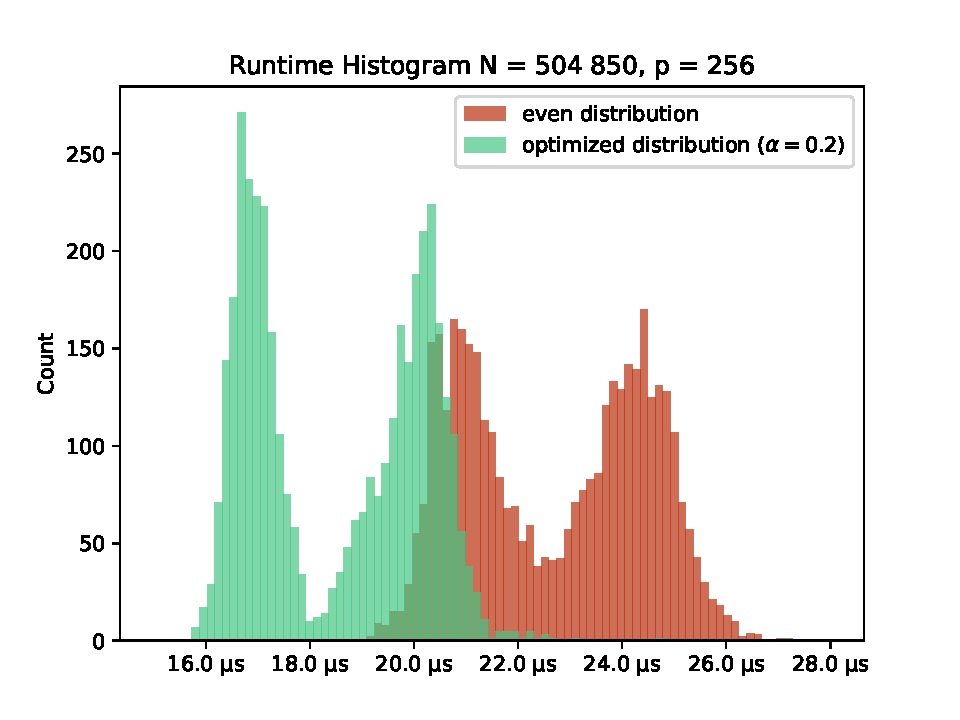
\includegraphics[scale=0.75]{figures/distribution_experiment}
\caption{Runtime comparison of even vs.\ optimized data distribution}
\label{fig:distribution_runtimes}
\end{figure}

\begin{figure}
\centering
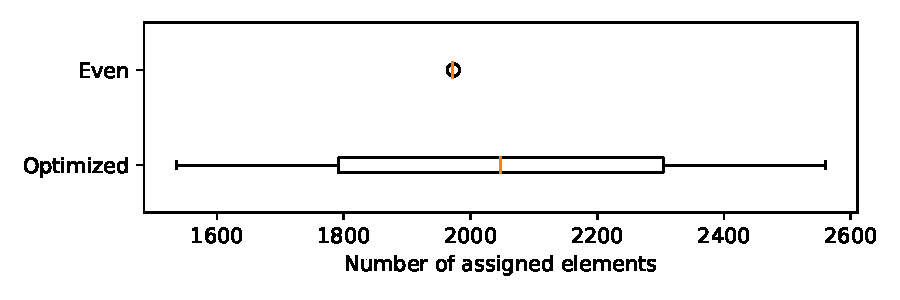
\includegraphics[scale=0.75]{figures/optimizedDistributionBoxplot.pdf}
\caption{Boxplot of the assigned number of elements per \gls{pe} for the even and optimized data distribution.}
\label{fig:distributionBoxplot}
\end{figure}


\subsubsection{Drawbacks of the Scoring Function}
\label{sec:ScoringFunctionDrawbacks}
The scoring function \eqref{eq:distributionScore} has two major drawbacks:
it does not consider the critical path of calculations and also assumes that the time $t_\textrm{MPI\_Send}$ is constant.
This causes a discrepancy between predicted score times and measured benchmark times.
Nonetheless, it provides a runtime model accurate enough so that distributions with a better score perform better under benchmark conditions.


\subsection{Index-lookup Hashmap}
\label{sec:IndexLookupHashmap}

\begin{figure}
\centering
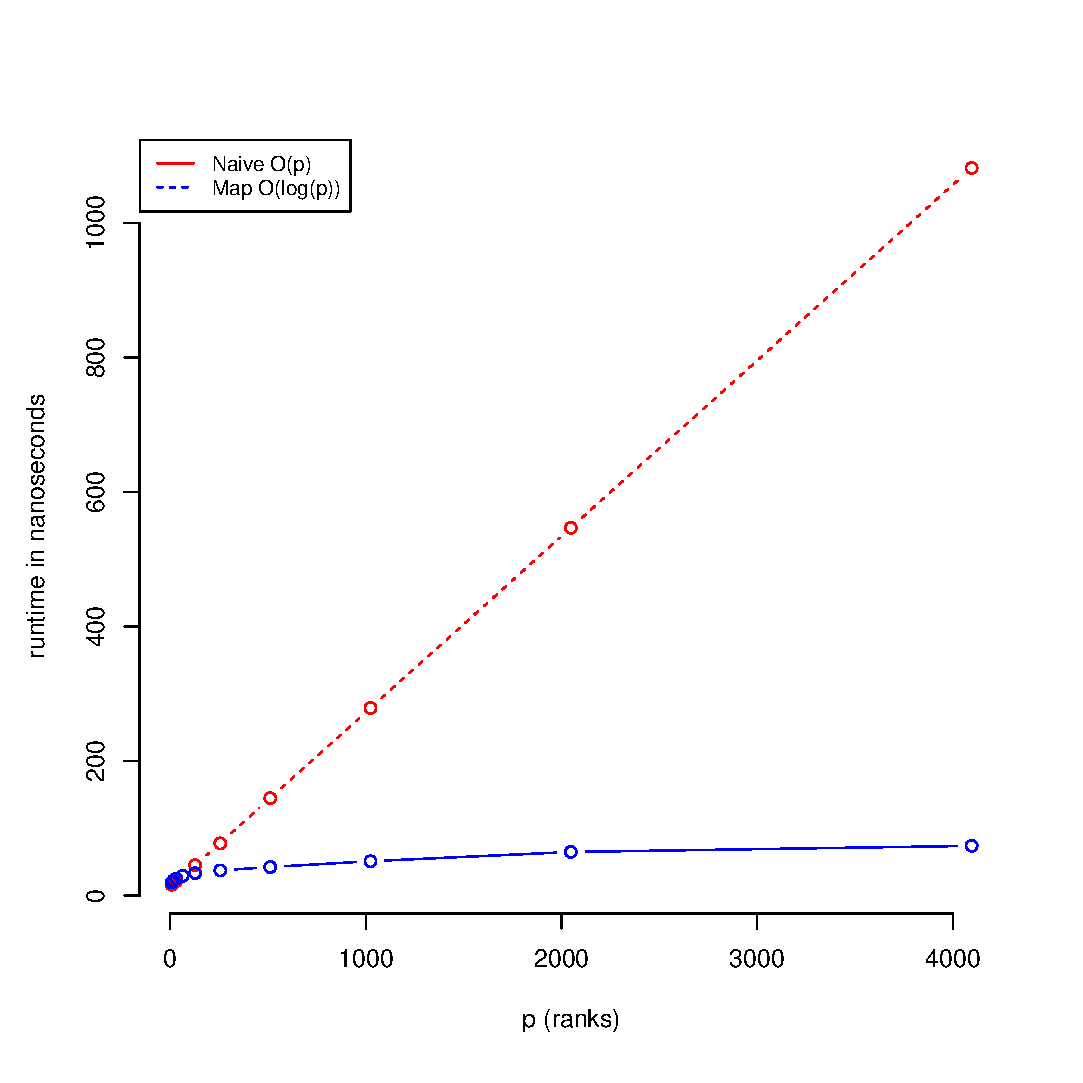
\includegraphics[scale=0.55]{figures/microbenchmark_rank_from_index.eps}
\caption{Microbenchmark comparison of unoptimized and optimized $\rankFromIndex$ function}
\label{fig:microbenchmarkRankFromIndex}

\end{figure}

\Cref{algo:SummationAlgo} uses the $\rankFromIndex$ function to lookup the \gls{pe}-rank for a given element index.
This function maps the binary tree structure to the underlying computing topology and its execution speed is performance-critical due to its position inside a frequently executed loop.

The initial implementation used a loop to find the first entry in the \textit{startIndices} array which numerically exceeds the input index.
The runtime of this algorithm is $O(p)$.
Microbenchmarks revealed the linearly increasing runtime and the need for optimization (see \Cref{fig:microbenchmarkRankFromIndex}).
The currently implemented version uses a map (\texttt{std::map}) to scan for the start index, which yields a runtime in $O(\log(p))$.

For $p=256$ \glspl{pe}, a single call to $\rankFromIndex$ takes about \SI{620}{\micro\second}.
With $N = 1\,327\,505$ elements, \Cref{algo:SummationAlgo} calls $\rankFromIndex$ $1913$ times, about $7$ times per \gls{pe}.
Thus, the $\rankFromIndex$ calculation takes up about \SI{4.3}{\micro\second} of the total accumulation time of \SI{30.5}{\micro\second}, suggesting that further optimization could offer a $15\%$ performance gain.
\subsection{Vectorization}
\label{sec:Vectorization}

\begin{figure}
\begin{tikzpicture}[
block/.style={draw,minimum width=1.6cm, text centered,minimum height=0.8cm,font=\small}]

\node[block,left=0.8cm of {0,0}](d){$D$};
\node[block,left=0cm of d](c){$C$};
\node[block,left=0cm of c](b){$B$};
\node[block,left=0cm of b](a){$A$};




\node[block,right=0.8cm of {0,0}](e){$E$};
\node[block,right=0cm of e](f){$F$};
\node[block,right=0cm of f](g){$G$};
\node[block,right=0cm of g](h){$H$};



\node[block,below=2cm of {-2.4,0}](ab){$A+B$};
\node[block,right=0cm of ab](ef){$E+F$};
\node[block,right=0cm of ef](cd){$C+D$};
\node[block,right=0cm of cd](gh){$G+H$};

\node[below=0.8cm of {0,0}](op1) {$\_mm256\_hadd\_pd$};
\path[->,very thick] (c) edge (-1.6,-2);
\path[->,very thick] (f) edge (1.6,-2);

\node[block,below=4cm of c](ab2){$A+B$};
\node[block,right=0cm of ab2](ef2){$E+F$};
\node[block,below=4cm of e](cd2){$C+D$};
\node[block,right=0cm of cd2](gh2){$G+H$};
\path[->,very thick] (-1.6,-2.8) edge (-2.4,-4.4);
\path[->,very thick] (1.6,-2.8) edge (2.4,-4.4);
\node[left=0.6cm of {-2.0,-3.6}] (op2) {$\_mm256\_extractf128\_pd$};
\node[right=0.6cm of {2.0,-3.6}] (op3) {$\_mm256\_castpd256\_pd128$};

\node[block,left=0cm of {0,-7}](abcd){$(A+B)+(C+D)$};
\node[block,right=0cm of abcd](efgh){$(E+F)+(G+H)$};
\path[->,very thick] (-2.4,-5.2) edge (-2,-6.6);
\path[->,very thick] (2.4,-5.2) edge (2,-6.6);
\node[above=0.4cm of {0,-6.6}](op4) {$\_mm\_add\_pd$};

\node[block,left=0cm of {0,-9}](abcdefgh){$((A+B)+(C+D))+((E+F)+(G+H))$};
\node[block,right=0cm of abcdefgh](abcdefgh2){$((A+B)+(C+D))+((E+F)+(G+H))$};
\path[->,very thick] (0,-7.4) edge (0,-8.6);
\node[right=0.4cm of {0,-8}](op5) {$\_mm\_hadd\_pd$};

\end{tikzpicture}
\caption{Register content during AVX-2 subtree summation}
\label{fig:avxSchema}
\end{figure}

\begin{figure}
\centering
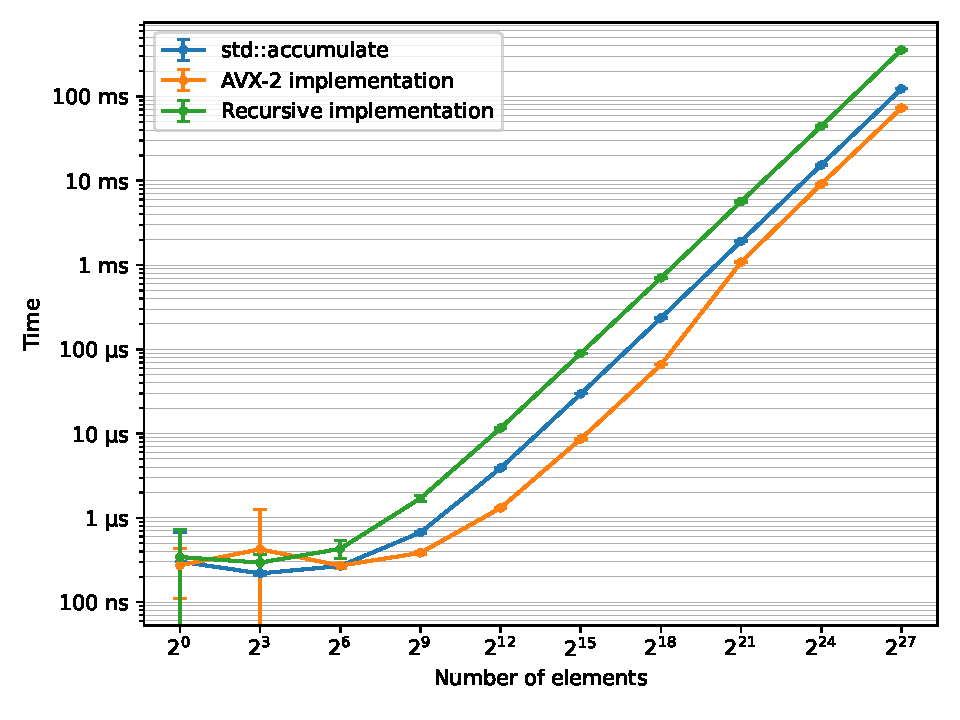
\includegraphics[scale=0.72]{figures/benchmarkVectorization}
\caption{Microbenchmark comparing sequential summation to AVX-2 binary tree reduction for $p=1$}
\label{fig:benchmarkVectorization}
\end{figure}

The theoretical per-node peak of \gls{flops} increases dramatically under the utilization of \gls{simd} capabilities~\cite{dolbeau_theoretical_2018}.
While modern compilers like the GNU C-Compiler try to automatically vectorize existing code\footnote{We confirmed manually that the relevant code sections compile to AVX machine instructions after passing the \texttt{-mavx} flag}, optimization by hand can yield better results.

Compared to the simple left-to-right reduction presented in \Cref{sec:SequentialLeftToRightReduction}, a reduction tree lends itself better to parallelization, since an algorithm can reduce subtrees independently.
Our implementation uses x86 \gls{avx}, specifically AVX-2.
AVX-2 registers are $256$ bits wide and can therefore store four double precision floating-point numbers.
\Cref{algo:AVXTreeAccumulation} uses two registers to accumulate a subtree of eight elements at once.
Because AVX-2 instructions manipulate data within 128-bit lanes, it is necessary to extract the upper 128-bit after the first horizontal add in order to follow the correct summation order.
\Cref{fig:avxSchema} displays the register contents over time.
\begin{algorithm}
\caption{8-tree summation with AVX-2 instructions}
\label{algo:AVXTreeAccumulation}
\DontPrintSemicolon
\SetAlgoLined
\KwData{Buffer \textit{buffer} with at least $8$ entries at offset $i$}
\KwResult{Subtree sum of $8$ elements}

$a \gets mm256\_load\_pd(buffer[i])$\;
$b \gets mm256\_load\_pd(buffer[i + 4])$\;
$level1Sum \gets mm256\_hadd\_pd(a,b)$\;

$c \gets mm256\_extractf128\_pd(level1Sum 1)$\;
$d \gets mm256\_castpd256\_pd128(level1Sum)$\;
$level2Sum \gets mm\_add\_pd(c, d)$\;

$level3Sum \gets mm\_hadd\_pd(level2Sum, level2Sum)$\;

\Return $mm\_cvtsd\_f64(level3Sum)$\;
\end{algorithm}

Our implementation uses \Cref{algo:AVXTreeAccumulation} as a subroutine inside \Cref{algo:SummationAlgo} to advance the iterative reduction three levels per iteration.
If the remaining number of elements in the current iteration is not divisible by eight, the algorithm processes the remaining elements using non-vectorized instructions.
\Cref{fig:benchmarkVectorization} compares the runtime of three accumulation algorithms: the initial recursive implementation of binary tree reduction, the vectorized AVX-2 implementation and the \texttt{std::accumulate} routine from the C++ standard library.
Since only one \gls{pe} executes this microbenchmark, no communication takes place and all runtime costs are purely computational.
For smaller workloads ($N < 64$), the overhead introduced by the vectorization is larger than the performance gains, but for larger workloads the AVX-2 implementation outperforms \texttt{std::accumulate} by a factor of more than $2$.
\texttt{std::accumulate} guarantees the summation order to be left-to-right and therefore can not be vectorized.

\chapter{Experiments}
\label{ch:Experiments}

In this chapter, we will compare the runtimes of three summation procedures:
\begin{itemize}
  \item the binary tree summation algorithm as presented in chapters \ref{ch:BinaryTreeSummation} and \ref{ch:Implementation}
  \item the ReproBLAS reduce operation
  \item a bitwise-irreproducible implementation with \texttt{MPI\_Allreduce} and \texttt{std::accumulate} as baseline.
\end{itemize}

\section{Experimental Setup}
\label{sec:ExperimentalSetup}
The machine \textit{i10pc138}, which has two AMD EPYC 7713 CPUs with $64$ cores each, $2$ threads per core for a total of $256$ CPUs and $1024$ GB of DDR4 main memory, executed all benchmarks with less than $257$ \glspl{pe}.
The bwUniCluster 2.0 ran all other benchmarks.

\begin{table}
\centering
\begin{tabular}{r|l}
\textbf{dataset name} & \textbf{number of summands} \\
354 & $460$ \\
multi100 & $767$ \\
prim & $898$ \\
fusob & $1\,602$ \\
dna\_rokasD4 & $239\,763$ \\
aa\_rokasA8 & $504\,850$ \\
dna\_rokasD1 & $1\,327\,505$ \\
aa\_rokasA4 & $1\,806\,035$ \\
dna\_PeteD8 & $3\,011\,099$ \\
dna\_rokasD7 & $21\,410\,970$ \\
\end{tabular}
\caption{Overview of benchmark datasets}
\label{table:datasets}
\end{table}

Input data was extracted from RAxML-NG workloads in the form of an array of double-precision floating point numbers representing per-site log-likelihood values.
The datasets come in various sizes, depending on the multiple sequence alignment length. Table \ref{table:datasets} gives an overview.
Each benchmark run performs the following steps for each summation mode (\texttt{reproblas}, \texttt{allreduce}, \texttt{tree}) and each dataset:
\begin{enumerate}
\item Load input data from file and distribute it among the \glspl{pe}
\item Perform the summation $100$ times, measuring the duration for each time
\item Prune the first and last eight measurements
\end{enumerate}

\section{Results}
\label{sec:Results}

\begin{figure}
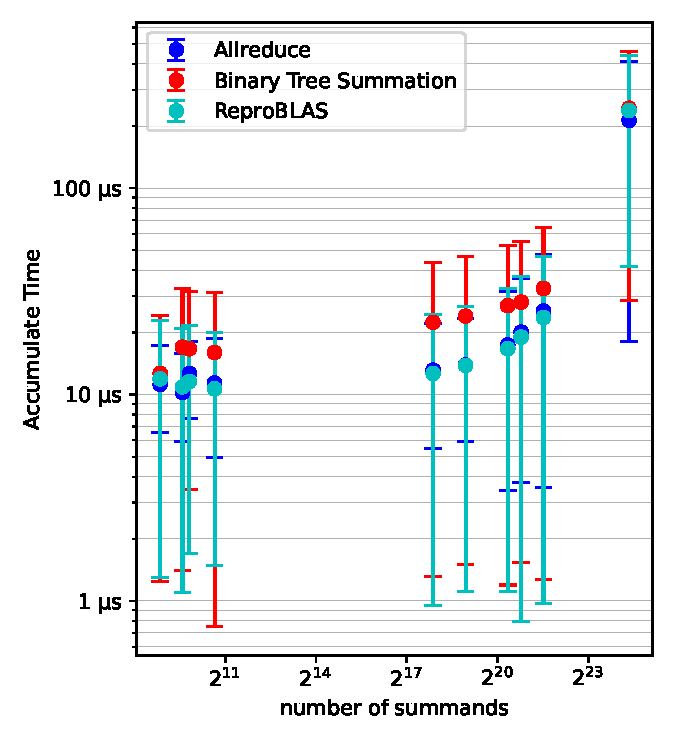
\includegraphics[scale=1]{figures/benchmarkScatter.pdf}
\caption{Summation runtime for different datasets across $256$ \glspl{pe}}
\label{fig:benchmarkOverview}
\end{figure}

\begin{figure}
\centering
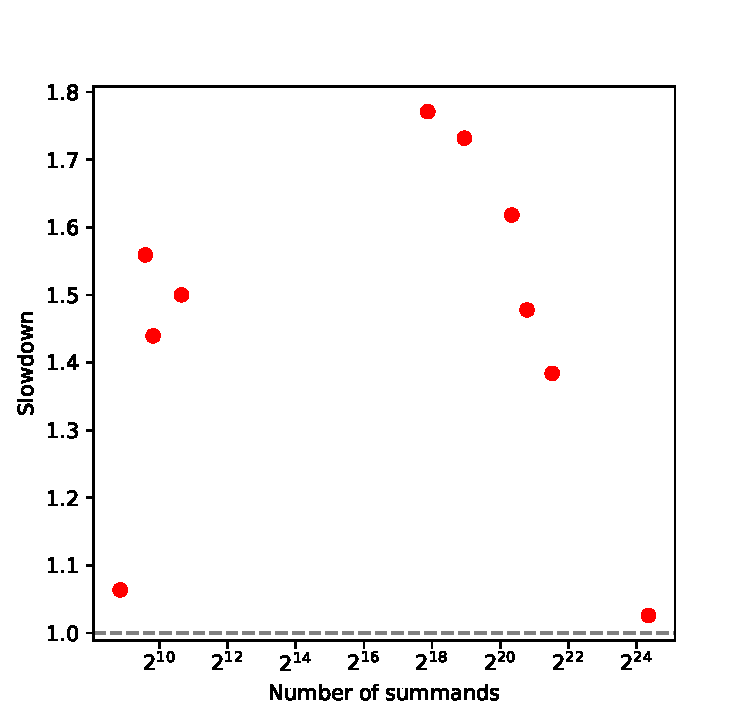
\includegraphics[scale=0.8]{figures/slowdownPlot.pdf}
\caption{Relative slowdown of binary tree summation compared to ReproBLAS}
\label{fig:slowdownPlot}
\end{figure}

Figure \ref{fig:benchmarkOverview} shows the runtime measurements across all datasets as scatter plot.
Error bars depict the standard deviation of measurements.
All measured summation algorithms have a runtime that is linear in the number of summands. For most datasets, ReproBLAS is faster than Allreduce and Allreduce is faster than binary tree summation.

Figure \ref{fig:slowdownPlot} shows the exact relative slowdown of binary tree summation compared to ReproBLAS.
While the slowdown on small datasets varies greatly (presumably due to the chaotic message count behaviour discussed in section \ref{sec:messageCount}), for larger datasets the slowdown approaches $1$, meaning binary tree summation is almost as fast as ReproBLAS.
Figure \ref{fig:violinRokasD7} shows the exact distribution of runtimes for the largest dataset.


\begin{figure}
\centering
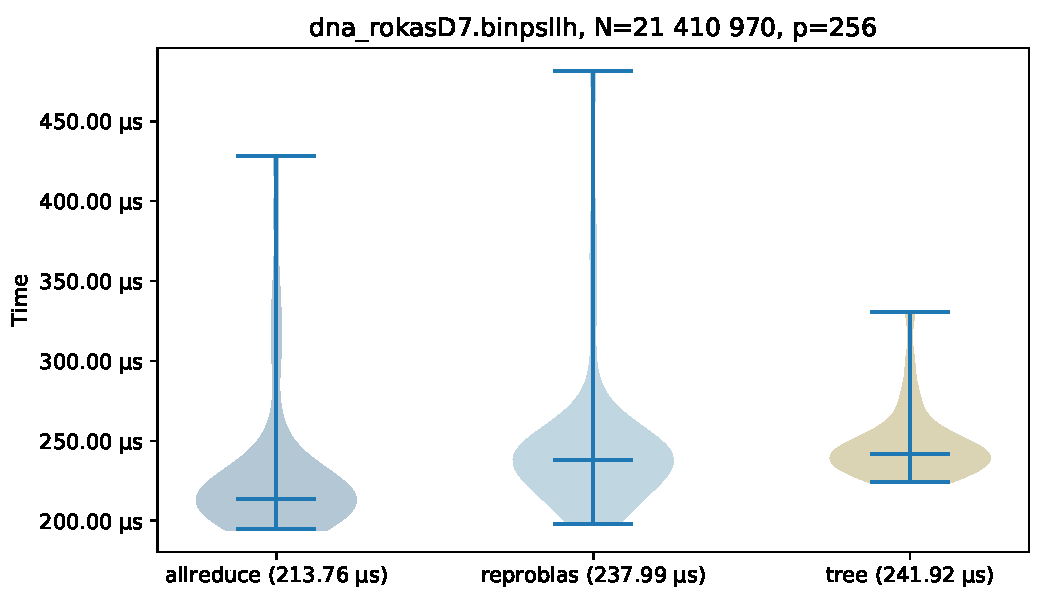
\includegraphics[scale=0.8]{figures/violinRokasD7.pdf}
\caption{Runtime distribution for all three summation modes on the dataset \textit{rokasD7}}
\label{fig:violinRokasD7}
\end{figure}


\section{Verification of Reproducibility}
\label{sec:VerificationOfReproducibility}

\section{Scaling Behaviour}
\label{sec:ScalingBehaviour}
%% LaTeX2e class for student theses
%% sections/evaluation.tex
%% 
%% Karlsruhe Institute of Technology
%% Institute for Program Structures and Data Organization
%% Chair for Software Design and Quality (SDQ)
%%
%% Dr.-Ing. Erik Burger
%% burger@kit.edu
%%
%% Version 1.3.5, 2020-06-26

\chapter{Discussion}
\label{ch:Discussion}

%% LaTeX2e class for student theses
%% sections/conclusion.tex
%% 
%% Karlsruhe Institute of Technology
%% Institute for Program Structures and Data Organization
%% Chair for Software Design and Quality (SDQ)
%%
%% Dr.-Ing. Erik Burger
%% burger@kit.edu
%%
%% Version 1.3.5, 2020-06-26

\chapter{Conclusion}
\label{ch:Conclusion}

Binary Tree Reduction offers reproducible results independent of the core-count.
It is not limited to floating-point operations and can be extended to the general set of reduction operations.
Its message count per \gls{pe} is bounded logarithmically by the number of elements per \gls{pe} (Equation \ref{eq:upperBoundLowerDistribution}).
If the Binary Tree Reduction takes up the majority of the runtime, optimizing the data distribution for the reduction can yield better results (\Cref{sec:DataDistribution}).

For floating-point summation in particular, solutions like ReproBLAS~\cite{ahrens_algorithms_2020} outperform Binary Tree Reduction and have a negligible runtime penalty compared to naive \texttt{MPI\_Allreduce} implementations.
The slowdown of Binary Tree Reduction compared to ReproBLAS is typically less than $2$.

Future work could explore additional optimizations of the Binary Tree Reduction algorithm.
Under the assumption of a specific data distribution, $\rankFromIndex$-lookups could be replaced with a constant time algorithm.
Furthermore, critical path analysis could provide better-performing calculation orders for outbound subtree roots.
While \Cref{ch:Experiments} provides insight in the runtime of isolated reduction operations, additional examinations must be made to determine the runtimes of reductions which are a small part of larger workloads.

%% --------------------
%% |   Bibliography   |
%% --------------------

%% Add entry to the table of contents for the bibliography
\printbibliography[heading=bibintoc]

%% ----------------
%% |   Appendix   |
%% ----------------
\appendix
%% LaTeX2e class for student theses
%% sections/apendix.tex
%% 
%% Karlsruhe Institute of Technology
%% Institute for Program Structures and Data Organization
%% Chair for Software Design and Quality (SDQ)
%%
%% Dr.-Ing. Erik Burger
%% burger@kit.edu
%%
%% Version 1.3.5, 2020-06-26

\chapter{Glossary}
\printglossary[type=\acronymtype]
\printglossary

\iflanguage{english}
{\chapter{Appendix}}    % english style
{\chapter{Anhang}}      % german style
\label{chap:appendix}



%% -------------------
%% | Example content |
%% -------------------
\section{First Appendix Section}
\label{sec:appendix:FirstSection}
		
\setcounter{figure}{0}
		
\begin{figure} [ht]
  \centering
  \caption{A figure}
  \label{fig:anotherfigure}
\end{figure}


\dots
%% ---------------------
%% | / Example content |
%% ---------------------

\end{document}
